\documentclass[14pt, a4paper]{extarticle}
\usepackage{GOST}
\usepackage{array}
\usepackage{verbatim}
\usepackage[detect-all]{siunitx}
\usepackage{amsmath}
\usepackage{amssymb}
\usepackage[utf8]{inputenc}
\usepackage{hyperref}

\usepackage{ifthen}


\usepackage{tempora}


\makeatletter
\renewcommand\@biblabel[1]{#1.}
\makeatother

% Для листинга кода:
\usepackage{listings}
\lstset{ %
	language=python,                 % выбор языка для подсветки (здесь это С)
	basicstyle=\small\sffamily, % размер и начертание шрифта для подсветки кода
	numbers=left,               % где поставить нумерацию строк (слева\справа)
	numberstyle=\tiny,           % размер шрифта для номеров строк
	stepnumber=1,                   % размер шага между двумя номерами строк
	numbersep=5pt,                % как далеко отстоят номера строк от подсвечиваемого кода
	showspaces=false,            % показывать или нет пробелы специальными отступами
	showstringspaces=false,      % показывать или нет пробелы в строках
	showtabs=false,             % показывать или нет табуляцию в строках
	frame=single,              % рисовать рамку вокруг кода
	tabsize=2,                 % размер табуляции по умолчанию равен 2 пробелам
	captionpos=t,              % позиция заголовка вверху [t] или внизу [b] 
	breaklines=true,           % автоматически переносить строки (да\нет)
	breakatwhitespace=false, % переносить строки только если есть пробел
	escapeinside={\#*}{*)}   % если нужно добавить комментарии в коде
}


%для графиков
\usepackage{pgfplots}
\usepackage{filecontents}
\usetikzlibrary{datavisualization}
\usetikzlibrary{datavisualization.formats.functions}

\begin{document}
	
	\begin{table}[ht]
		\centering
		\begin{tabular}{|c|p{400pt}|} 
			\hline
			\begin{tabular}[c]{@{}c@{}} 
\includegraphics[scale=1]{baum.jpg} \\\end{tabular} &
			\footnotesize\begin{tabular}[c]{@{}c@{}}\textbf{Министерство~науки~и~высшего~образования~Российской~Федерации}\\\textbf{Федеральное~государственное~бюджетное~образовательное~учреждение}\\\textbf{~высшего~образования}\\\textbf{«Московский~государственный~технический~университет}\\\textbf{имени~Н.Э.~Баумана}\\\textbf{(национальный~исследовательский~университет)»}\\\textbf{(МГТУ~им.~Н.Э.~Баумана)}\\\end{tabular}  \\
			\hline
		\end{tabular}
	\end{table}
	\noindent\rule{\textwidth}{4pt}
	\noindent\rule[14pt]{\textwidth}{1pt}
	\hfill 
	\noindent
	\makebox{ФАКУЛЬТЕТ~}%
	\makebox[\textwidth][l]{\underline{~«Информатика и системы управления»~~~~~~~~~~~~~~~~~~~~~~~~~~~~~~~~~}}%
	\\
	\noindent
	\makebox{КАФЕДРА~}%
	\makebox[\textwidth][l]{\underline{~«Программное обеспечение ЭВМ и информационные технологии»~}}%
	
	
	\begin{center}
		\vspace{1.5cm}
		{\bf\huge Отчёт\par}
		{\bf\Large по лабораторной работе № 1\par}
		\vspace{0.7cm}
	\end{center}
	
	
	\noindent
	\makebox{\large{\bf Название:}~~~}
	\makebox[\textwidth][l]{\large\underline{Программная реализация приближенного~~~~~~~~~~~~~~~~~~~~}}
	\makebox[\textwidth][l]{\large\underline{аналитического метода и численных алгоритмов первого~~~~~~~~~~~~~~~~~}}
	\makebox[\textwidth][l]{\large\underline{и второго порядков точности при решении задачи Коши для ОДУ.~~}}
	
	\noindent
	\makebox{\large{\bf Дисциплина:}~~~}
	\makebox[\textwidth][l]{\large\underline{~Моделирование~~~~~~~~~~~~~~~~~~~~~~~~~~}}\\
	
	\vspace{1.5cm}
	\noindent
	\begin{tabular}{l c c c c c}
		Студент      & ~ИУ7-65Б~               & \hspace{2.5cm} & \hspace{2cm}                 & &  Д.В. 
		Сусликов \\\cline{2-2}\cline{4-4} \cline{6-6} 
		\hspace{3cm} & {\footnotesize(Группа)} &                & {\footnotesize(Подпись, дата)} & & {\footnotesize(И.О. Фамилия)}
	\end{tabular}
	
	\noindent
	\begin{tabular}{l c c c c}
		Преподаватель & \hspace{5cm}   & \hspace{2cm}                 & & ~~~~~~В.М. Градов~~~~~~\\\cline{3-3} \cline{5-5} 
		\hspace{3cm}  &                & {\footnotesize(Подпись, дата)} & & {\footnotesize(И.О. Фамилия)}
	\end{tabular}
	
	\vspace{0.6cm}
	\begin{center}	
		\vfill
		\large \textit {Москва, 2021}
	\end{center}
	
	\thispagestyle {empty}
	\pagebreak
	
	% СОДЕРЖАНИЕ 
	\clearpage
		
	% ВВЕДЕНИЕ
	\clearpage
	\section*{Введение}
	\addcontentsline{toc}{section}{Введение}
	\textbf{Цель работы:} Получение навыков решения задачи Коши для ОДУ методами Пикара и
	явными методами первого порядка точности (Эйлера) и второго порядка точности (Рунге-Кутта).\par
	\textbf{Исходные данные:}
	\par ОДУ, не имеющее аналитического решения\par
		$$u'(x) = x^2 + u^2, $$
		$$u(0) = 0 $$
	\par
	
	\textbf{Результат работы программы}
	\par Таблица, содержащая значения аргумента с заданным шагом в интервале [0, xmax] и
		результаты расчета функции u(x) в приближениях Пикара (от 1-го до 4-го), а также
		численными методами. Границу интервала xmax выбирать максимально возможной из
		условия, чтобы численные методы обеспечивали точность вычисления решения уравнения
		u(x) до второго знака после запятой. 
	\par
 
	\begin{enumerate}
		\item \textbf{Метод Пикара}
		
		$y^{(1)}=\frac{x^3}{3}\\$
		$y^{(2)}=\frac{x^3}{3} + \frac{x^7}{63}\\$
		$y^{(3)}=\frac{x^3}{3}+ \frac{x^7}{63} + \frac{2x^{11}}{2079} + \frac{x^{15}}{59535}\\$	
		$y^{(4)}=\frac{x^3}{3}+ \frac{x^7}{63} + \frac{2x^{11}}{2079} + \frac{13x^{15}}{218295} + \frac{82x^{19}}{37328445} +  \frac{662x^{23}}{10438212015}+\\ \frac{4x^{27}}{3341878155}+\frac{x^{31}}{109876902975}$
		
		\item \textbf{Метод Эйлера}\par
		$y_{n+1}=y_n+h\cdot f(x_n,y_n)\text{ , где }f(x,y)=x^2+y^2$
		
		\newpage
		\item \textbf{Метод Рунге-Кутта}\par
		$y_{n+1}=y_n+h\cdot((1 - \alpha)k_1 + \alpha k_2), где\\
		k_1 = f(x_n, y_n)\\
		k_2 = f(x_n + \frac{h}{2 \alpha}, y_n + \frac{h}{2 \alpha}k_1),\\
		\alpha = \frac{1}{2} \text{ or } 1$
			
	\end{enumerate}
	
	\textbf{Результаты}\par
	Ниже приведены результаты расчёта функции u(x) с шагом  $10^{-5}$
	и значением $\alpha$ = 1 в методе Рунге-Кутта.
	
	\begin{figure}[h!]
		\centering{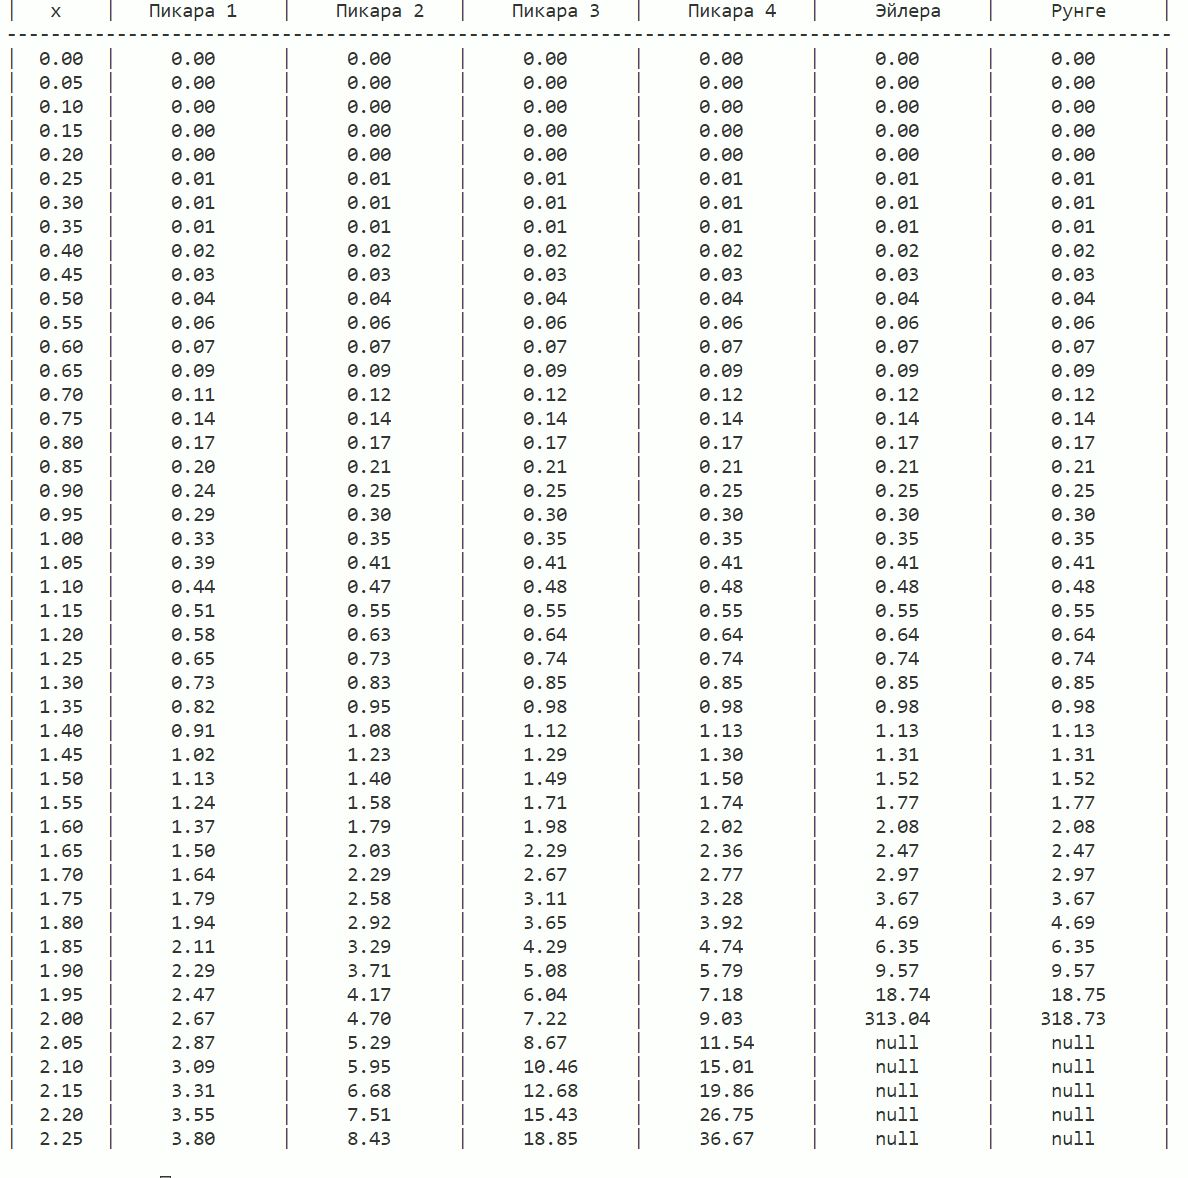
\includegraphics[scale=0.7]{res.jpg}}
	\end{figure}
	
	\newpage
	
	
	\section*{Ответы на вопросы}
	\begin{enumerate}
		\item[1)] \textbf{Вопрос:} Укажите интервалы значений аргумента, в которых можно считать решением заданного уравнения каждое из первых 4-х приближений Пикара. Точность результата оценивать до
		второй цифры после запятой. Объяснить свой ответ.
			
		\textbf{Ответ:} При оценке значений до 2-й цифры после запятой общим интервалом, где совпадают значения у всех приближений Пикара, будет [0, 65]. Если оценивать по отдельности, то для 1-го - [0, 65], 
		для 2-го - [0, 1.05], для 3-го - [0, 1.4], для 4-го - [0, 1.4].
			
		Интервалы для 3-его и 4-ого приближения одинаковые из-за того, что
		нельзя гарантировать, что 4-ое приближение вычисляется правильно, так как для этого
		нужно приближение более высокого порядка.
		
		Интервалы разнятся, так как чем больше приближение, тем точнее результат.
		
		\item[2)] \textbf{Вопрос:} Пояснить, каким образом можно доказать правильность полученного результата при
		фиксированном значении аргумента в численных методах.
		
		\textbf{Ответ:} Численные методы работают пошагово, поэтому точность полученного результата зависит от величины шага. То есть, чтобы доказать правильность результата нужно вычислять значения сперва с большим шагом, постепенно уменьшая его, до тех пор, пока изменение результата будет пренебрежительно мало. Итоговый результат можно считать верным. Приведу пример вычисления значения u(2):
		\par
		\begin{table}[h]
			\begin{tabular}{|l|l|l|}\hline
				шаг    & Метод Эйлера  & Метод Рунге\\ \hline
				$10^{-2}$ & 36.49  & 575.95 \\
				$10^{-3}$ & 142.63  & 420.29 \\
				$10^{-4}$ & 277/36  & 327.89 \\
				$10^{-5}$ & 313.04  & 318.73 \\
				$10^{-6}$ & 317.25  & 317.82 \\
				\hline     
			\end{tabular}
		\end{table}
		
		
		\newpage
		\item[3)] \textbf{Вопрос:} Каково значение функции при x=2, т.е. привести значение u(2).
		\textbf{Ответ:} 
		\par
		\begin{table}[h]
			\begin{tabular}{|l|l|l|}\hline
				x    & Метод  & Метод \\
				& Эйлера  & Рунге \\ \hline
				2.00 & 317.25  & 317.82 \\
				\hline     
			\end{tabular}
		\end{table}
	\end{enumerate}
	
	\textbf{Код программы}

	\begin{lstlisting}[caption=Метод Эйлера]
		def euler(h, x):
			y = 0
			x0 = h
			while (x0 < x + h / 2):
			try:
				y += h * func(x0, y)
				x0 += h
			except:
				return 'null'
		
			return y
	\end{lstlisting}


	\begin{lstlisting}[caption=Метод Рунге-Кутта]
		def runge(h, x):
			alpha = 1
			y = 0
			x0 = h
			while (x0 < x + h / 2):
			try:
				k1 = func(x0, y)
				k2 = func(x0 + h / 2 / alpha, y + h / 2 / alpha * k1)
				y += h * ((1 - alpha) * k1 + alpha * k2)
				x0 += h
			except:
				return 'null'
			
			return y
	\end{lstlisting}

	\begin{lstlisting}[caption=Метод Пикара]
		def approximation1(arg):
			return arg ** 3 / 3
		
		def approximation2(arg):
			return approximation1(arg) + arg ** 7 / 63
		
		def approximation3(arg):
			return approximation2(arg) + (arg ** 11) * (2 / 2079) + (arg ** 15) / 59535
		
		def approximation4(arg):
			return approximation3(arg) + (arg ** 15)*(2 / 93555) + (arg ** 19)*(2 / 3393495) + \
			(arg ** 19)*(2 / 2488563) + (arg ** 23)*(2 / 86266215) + (arg ** 23)*(1 / 99411543) + \
			(arg ** 27)*(2 / 3341878155) + (arg ** 31)*(1 / 109876902975)
		
		def picar(x):
			y_approx1 = approximation1(x)
			y_approx2 = approximation2(x)
			y_approx3 = approximation3(x)
			y_approx4 = approximation4(x)
		
			return [y_approx1, y_approx2, y_approx3, y_approx4]
	\end{lstlisting}
	\newpage
	
\end{document}